\documentclass[12pt, a4paper, titlepage]{report}
\usepackage[a4paper,top=2.5cm,bottom=2cm,left=2cm,right=2cm]{geometry}
\usepackage[italian]{babel}
\usepackage[hidelinks]{hyperref}
\usepackage{graphicx}
\usepackage{algorithm}
\usepackage{capt-of}
\usepackage{amsmath}
\usepackage{longtable}
\usepackage{caption}
\usepackage{booktabs}
\usepackage{algpseudocode}
\usepackage{makecell}
\usepackage[utf8]{inputenc}
\usepackage{fixltx2e}
\usepackage{listings}
\usepackage{hyperref}
\usepackage{makecell}
\usepackage{changepage}
\usepackage{paracol}
\usepackage{siunitx}
\usepackage{lipsum}
\usepackage{float}
\usepackage{subfig}

\usepackage[swapnames]{frontespizio}

\usepackage{fancyhdr}
\usepackage{lastpage}
%\pagestyle{fancy}
%\fancyhf{}
%\cfoot{Pagina \thepage\ di \pageref{LastPage}}

\setcounter{tocdepth}{6}
\setcounter{secnumdepth}{6}
\newcommand\tab[1][1cm]{\hspace*{#1}}
\renewcommand{\thesection}{\arabic{section}}%
\newcommand{\myparagraph}[1]{\paragraph{#1}\mbox{} \mbox{}}
\newcommand{\tommaso}{Tommaso Carraro}
\newcommand{\alberto}{Alberto Bezzon}
	
\begin{document}
	
	\begin{frontespizio}
		\begin{Preambolo*}
			\usepackage{fourier}
		\end{Preambolo*}
		\Universita{Padova}
		\Dipartimento{Matematica}
		\Scuola{Corso di Mobile Programming and Multimedia}
		\Filigrana [height=7.5cm,before=0.28,after=1]{logo-unipd.png}
		\Titolo{\vspace{8cm}\Huge{Relazione del progetto SmartOrder}}
		\Relatore{Alberto Bezzon 1211016\\Tommaso Carraro }
		\NRelatore{Studenti}{}
		\Annoaccademico{2018-2019}
	\end{frontespizio}
	
	%\maketitle
	%\pagestyle{empty}
	\setcounter{page}{2}
	\tableofcontents
	\newpage
	\listoffigures
%	\newpage
%	\listoftables
%	\setcounter{table}{0}
	\newpage	    
	\renewcommand*{\arraystretch}{2}
	\pagestyle{fancy}
	\fancyhf{}
	\rhead{Relazione del progetto SmartOrder}
	\lhead{Corso di Mobile Programming and Multimedia \\ Università di Padova}
	\cfoot{\thepage}
	%\setlength{\headsep}{2cm}
	
	\section{Introduzione}
	
	Il progetto consiste nello sviluppo di un'applicazione mobile, chiamata SmartOrder, progettata per permettere agli utenti registrati di effettuare ordini presso il proprio fornitore. L'applicazione è stata sviluppata esclusivamente per smartphone, al momento soltanto per l'ambiente Android, utilizzando il framework cross-platform PhoneGap. Per l'ambiente iOS è stato realizzato il progetto per XCode ma non essendo il gruppo in possesso di un Mac, non è stato possibile realizzare la versione iOS di SmartOrder. L'applicazione non prevede una registrazione esplicita, infatti le aziende che intendono acquistare il servizio devono comunicarlo al team di SmartOrder. Al momento della richiesta devono essere fornite le anagrafiche degli utenti che il fornitore intende registrare e in questo modo verranno creati gli account per tutti gli utenti, compresi di credenziali. Inoltre devono essere forniti i dati relativi a tutti gli articoli che il fornitore desidera rendere disponibili per gli utenti tramite il servizio. Una volta ricevute le credenziali, via mail, gli utenti possono iniziare ad usufruire del servizio. Il tutto sarà perfettamente configurato per fare in modo che ogni utente veda solamente gli articoli venduti dal proprio fornitore. Tramite l'applicazione sarà possibile:
	\begin{itemize}
		\item ricercare prodotti e aggiungerli al carrello;
		\item scansionare il codice a barre di un prodotto che si ha già acquistato per aggiungerlo al carrello più velocemente;
		\item modificare o eliminare i prodotti in carrello;
		\item inviare un ordine presso il proprio fornitore;
		\item visualizzare le informazioni relative a tutti gli ordini effettuati presso il proprio fornitore.
	\end{itemize}
	L'idea è nata per cercare di soddisfare un bisogno reale che proviene dallo zio di uno dei membri del gruppo. È stato richiesto se fosse possibile velocizzare il processo di rifornimento di libri di una libreria una volta terminati. L'idea è che è possibile velocizzare questo processo scansionando il codice a barre di un libro quando si è a conoscenza del fatto che sta per terminare. La possibiltà di aggiungere gli articoli dall'inventario è stata implementata per permettere all'applicazione di essere robusta rispetto all'aggiunta di nuovi clienti, in quanto essi non avendo ancora acquistato prodotti non hanno la possibilità di scansionare il codice a barre per ordinare i prodotti.
	
	\section{La scelta del framework cross-platform}
	
	Il framework cross-platform scelto per lo sviluppo dell'applicazione è PhoneGap. La scelta è ricaduta su questo framework in quanto un membro del gruppo aveva già familiarità con le tecnologie offerte dallo stesso. Inoltre il framework non avrebbe richiesto l'apprendimento di nuove tecnologie per l'implementazione dell'applicazione, in quanto è possibile utilizzare le tecnologie web. Altre considerazioni sulla scelta del framwork sono state inserite nelle conclusioni di questa relazione.
	
	\section{Accorgimenti sulle tecnologie web}
	
	Siccome è stato scelto il \textit{framework PhoneGap}, il gruppo ha utilizzato i linguaggi \textit{HTML5}, \textit{CSS3} e \textit{JavaScript}. In particolare, \textit{HTML5} è stato scelto perché include un insieme di funzionalità che permettono di valorizzare le interfacce \textit{mobile}. Alcune di queste evidenziano come \textit{HTML5} sia già per sua natura orientato al \textit{mobile}. In particolare \textit{HTML5} fornisce \textit{API} per:
	\begin{itemize}
		\item \textbf{eventi \textit{touch}}: mentre i meccanismi di input nei PC consistono per lo più nella tastiera e nel mouse, nei dispositivi mobili quasi tutto passa per il \textit{touch screen}, e avere funzionalità comode per gestire questo strumento consente un'interazione più ricca e senza limitazioni per l'utente. Le gestualità da attuare su un \textit{display}, nel mondo \textit{mobile}, costituiscono un vero e proprio linguaggio fondamentale nella \textit{user experience};
		\item \textbf{controllo batteria}: considerata l'importanza rivestita dalle risorse energetiche, l'esistenza stessa di questa libreria nel linguaggio dimostra come il suo impiego sia particolarmente mirato al panorama \textit{mobile}.
	\end{itemize}
	
	Ciò che ha favorito la scelta di \textit{CSS3} sono state le \textit{media queries}. Esse permettono di definire regole stilistiche in base alla tipologia del mezzo di visualizzazione, delle sue dimensioni e della sua attuale disposizione (\textit{portrait} o \textit{landscape}). Ciò influisce non solo sull'aspetto esteriore degli elementi ma anche sul loro posizionamento e quindi sulla struttura stessa dell'interfaccia.
	
	Per quanto riguarda il linguaggio \textit{JavaScript} si è utilizzato \textit{JavaScript} puro, senza l'utilizzo di \textit{framework} o \textit{JQuery}. Una particolarità del linguaggio, detta \textit{AJAX}, ha reso possibile eseguire chiamate all'\textit{API} del servizio \textit{web} di \textit{SmartOrder}. \textit{AJAX}, acronimo di \textit{\textit{Asynchronous JavaScript and XML}}, è una tecnica di sviluppo \textit{software} per la realizzazione di applicazioni \textit{web} interattive (\textit{Rich Internet Application}). Lo sviluppo di applicazioni \textit{HTML} con \textit{AJAX} si basa su uno scambio di dati in \textit{background} fra \textit{web browser} e \textit{server}, che consente l'aggiornamento dinamico di una pagina \textit{web} senza esplicito ricaricamento da parte dell'utente.
	
	\section{Informazioni utili all'utilizzo dell'applicazione}
	
	Per poter utilizzare l'applicazione è necessario essere connessi ad Internet, in quanto l'applicazione scarica i dati da un server. Si fa presente che la connessione viene bloccata dalla rete Eduroam e Studenti.math.unipd.it dell'Università, quindi si consiglia di utilizzare altre reti per usufruire dell'applicazione. Per ricevere le e-mail al momento dell'invio dell'ordine è necessario che la propria mail sia certificata Amazon. Questo è un limite di Amazon AWS che può essere aggirato inviando una semplice richiesta ad AWS. Poiché non sarà possibile quindi ricevere la mail, viene di seguito fornito uno screen della stessa. La mail presenta due versioni, a seconda che debba essere inviata all'azienda o all'utente che ha effettuato l'ordine.
	
	\section{Progettazione frontend}
	
	Il frontend è stato realizzato mediante utilizzo di tecnologie web. HTML e CSS hanno predisposto l'interfaccia grafica, mentre JavaScript ha permesso di implementare la logica applicativa.
	Le pagine realizzate sono le seguenti:
	\begin{itemize}
		\item \textit{index.html};
		\item \textit{login.html};
		\item \textit{homepage.html};
		\item \textit{order.html};
		\item \textit{article.html};
		\item \textit{articles.html};
		\item \textit{newpage.html};
		\item \textit{inventory.html}.
	\end{itemize}
	Ad ognuna di queste pagine è associato un foglio di stile e un file Javascript; inoltre sono presenti un file CSS e un file Javascript generali. Nelle prossime sezioni vengono descritte le funzionalità di SmartOrder.
	
	\subsection{Login e tutorial}
	
	L'applicazione, una volta installata, è utilizzabile. All'avvio della stessa viene mostrata la pagina di login per accedere al servizio. In questa schermata devono essere inserite le credenziali fornite dal proprio fornitore in fase di registrazione. La pagina presenta una checkbox "Resta collegato" per evitare che ad ogni apertura dell'applicazione venga richiesto il login. In seguito al login, soltanto al primo avvio, viene mostrato un breve tutorial sul funzionamento dell'applicazione. In fondo al tutorial è presente un bottone che permette di iniziare ad utilizzare l'app. Nel caso in cui un utente si trovasse in difficoltà durante l'utilizzo dell'applicazione, è possibile trovare il tutorial nel menu della stessa. Completato il tutorial si viene reindirizzati al \textit{Carrello}.
	
	\subsection{Carrello}
	La pagina \textit{Carrello} è la pagina principale dell'applicazione e visualizza per ogni articolo in carrello la quantità decisa dall'utente, il prezzo e il prezzo parziale (prezzo unitario x quantità). Ogni articolo in carrello presenta due bottoni: 
	\begin{itemize}
		\item \textbf{MODIFICA}: permette di modificare l'articolo. Alla sua pressione si viene reindirizzati alla pagina per la modifica dell'articolo, dove è possibile modificarne la quantità. Una volta effettuata la modifica è necessario confermarla per apportarla definitivamente, premendo sul bottone "Conferma", oppure annullarla, tramite il bottone "Annulla";
		\item \textbf{ELIMINA}: permette di rimuovere l'articolo dal carrello. Se tale bottone viene premuto, verrà chiesta conferma prima di effettuare l'operazione. (La spiegazione del perché viene rimandata al capitolo sul mobile design).
	\end{itemize}
	In questa pagina è presente inoltre un footer contenente:
	\begin{itemize}
		\item il prezzo totale di tutti gli articoli inseriti nel carrello;
		\item un pannello di bottoni utilizzabili per la gestione del carrello:
		\begin{itemize}
			\item bottone \textit{Scan}: la spiegazione di questo pulsante è presente nella sezione successiva;
			\item bottone \textit{Elimina}: permette di svuotare il carrello. In seguito alla pressione viene chiesta conferma dell'azione;
			\item bottone \textit{Invia}: permette di inviare un ordine composto dagli articoli nel carrello. In seguito all'ordine si riceverà una mail di conferma contenente le informazioni relative all'ordine effettuato.
		\end{itemize}
	\end{itemize} 
	
	\subsubsection{Aggiunta di un articolo al carrello}
	È possibile aggiungere un articolo al carrello in due modi: 
	\begin{enumerate}
		\item tramite scansione del codice a barre in seguito alla pressione del bottone \textit{Scan} nella pagina \textit{Carrello}, accedibile dal menu dell'applicazione;
		\item dalla pagina \textit{Inventario}, accedibile tramite il menu dell'applicazione, selezionando l'articolo che si desidera aggiungere e inserendone la quantità nella pagina di aggiunta dell'articolo. Una volta immessa la quantità desiderata, è necessario premere su "Conferma" affinché l'articolo venga inserito nel carrello, oppure su "Annulla" per annullare l'inserimento del nuovo articolo. Nella pagina \textit{Inventario} è inoltre possibile ricercare un'articolo, per nome o per codice, digitando la chiave di ricerca nella textbox in alto.
	\end{enumerate}
	La pagina per l'aggiunta di un articolo, che presenta la stessa interfaccia grafica della pagina per la modifica di un articolo, contiene le seguenti informazioni:
	\begin{itemize}
		\item nome dell'articolo: visualizzato in alto alla pagina;
		\item descrizione dell'articolo: visualizzata subito dopo il nome;
		\item pannello per l'inserimento della quantità: le modalità di interazione con questo pannello sono spiegate nella sezione dedicata al mobile design;
		\item prezzo dell'articolo: visualizzato alla fine della pagina. Si tratta di un campo dinamico in quanto varia a seconda della quantità inserita.
	\end{itemize}
	\\ \textbf{Attenzione}: nel caso in cui si cercasse di aggiungere al carrello un articolo già presente in esso, il sistema mostrerà un messaggio nel quale chiederà se si vuole modificare la quantità dello stesso.
	
	\subsection{Visualizzazione ordini}
	Dal menu dell'applicazione è possibile accedere alla lista di tutti gli ordini effettuati premendo sulla voce \textit{Ordini}. Alla sua pressione si verrà reindirizzati alla pagina \textit{Ordini}, dove per ogni ordine, vengono mostrate le seguenti informazioni:
	\begin{itemize}
		\item codice: è il codice che identifica univocamente l'ordine;
		\item data: è la data in cui è stato effettuato l'ordine;
		\item totale: è il totale in euro dell'ordine.
	\end{itemize}. 
	E' possibile consultare la lista degli articoli acquistati in un determinato ordine, tramite il bottone "DETTAGLI", situato sulla destra di ogni ordine. Alla sua pressione si verrà reindirizzati alla pagina contenente le informazioni degli articoli ordinati:
	\begin{itemize}
		\item nome;
		\item quantità;
		\item prezzo;
		\item prezzo parziale.
	\end{itemize}
	\noindent In questa pagina è possibile inoltre modificare la visualizzazione degli ordini, ordinandoli per data, dal più recente al meno recente, oppure per prezzo crescente. Per selezionare la tipologia di ordinamento è presente una select in fondo alla pagina.
	
	\section{Mobile design}
	
	In questa sezione vengono descritte le scelte implementative effettuate ai fini di una corretta progettazione dell'interfaccia dell'applicazione. Questa sezione è suddivisa in varie sottosezioni e ognuna di esse descrive un'elemento dell'interfaccia e le motivazioni alla base della sua progettazione.
	
	La maggior parte delle pagine dell'applicazione sono progettate nel seguente modo:
	\begin{itemize}
		\item la parte superiore presenta il pulsante menu sulla sinistra e il titolo della pagina al centro;
		\item la parte centrale presenta il contenuto informativo;
		\item la parte inferiore presenta un footer che varia a seconda della pagina.
	\end{itemize}
	
	\subsection{Bottoni}
	
	\begin{figure}[H] 
		\centering
		\subfloat[Bottoni presenti nel footer della pagina carrello ]{
\includegraphics[width=0.4\columnwidth]{img/buttons-cart}}
		\hspace*{2cm}
		\subfloat[Bottoni presenti nel footer delle apgine aggiungi e modifica articolo]{
\includegraphics[width=0.4\columnwidth]{img/buttons-add}}
		\caption{Bottoni nel footer}
		\label{fig:buttons}
	\end{figure}
	Nelle pagine \textit{Carrello}, \textit{Modifica} e \textit{Aggiungi} sono presenti dei bottoni nella parte bassa dello schermo (Figura \ref{fig:buttons}). L'applicazione richiede una frequente modifica dei dati quindi i controlli sono stati posizionati in una zona semplice da raggiungere e, seguendo la regola "Content always on top", si è preferito inserire questi bottoni in basso, infrangendo così la convenzione che su Android i controlli devono essere posizionati nella parte alta dello schermo. 
	\begin{figure}[H] 
		\centering
		\subfloat[Bottoni nella pagina Carrello ]{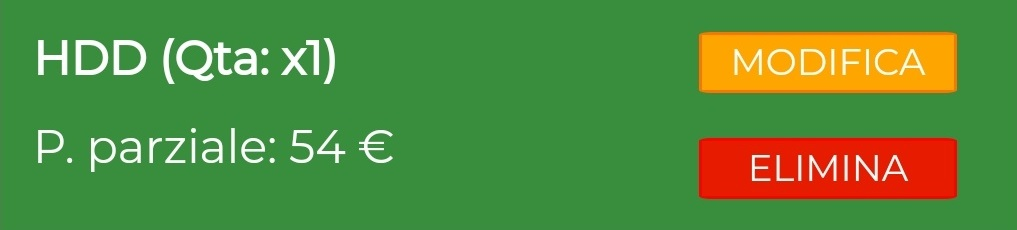
\includegraphics[width=0.3\columnwidth]{img/item-cart}}
		\hspace*{1cm}
		\subfloat[Bottoni nella pagina Ordini]{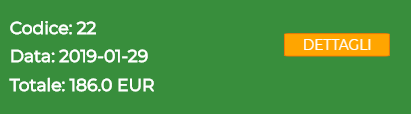
\includegraphics[width=0.3\columnwidth]{img/item-order}}
		\hspace*{1cm}
		\subfloat[Bottoni nella pagina Inventario]{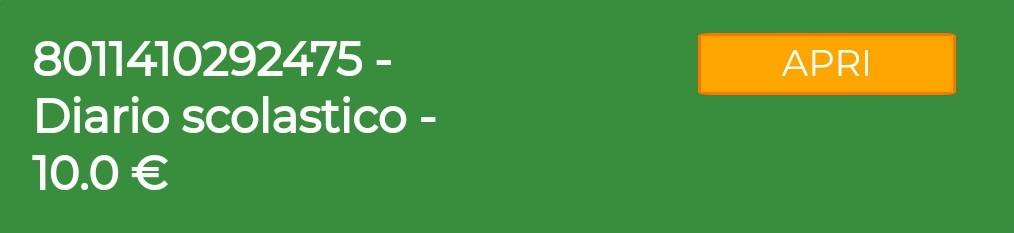
\includegraphics[width=0.3\columnwidth]{img/item-inventory}}
		\caption{Bottoni nella parte centrale delle pagine}
		\label{fig:item-buttons}
	\end{figure}
	\noindent I bottoni presenti in Figura \ref{fig:item-buttons} sono situati nella parte centrale dello schermo. Essendo disposti nella comfort zone sono facilmente raggiungibili e più piccoli rispetto ai bottoni del footer, in quanto si è seguita l'immagine in Figura \ref{fig:dimvspos}. La dimensione è stata opportunamente scelta per fare in modo che l'utente non prema accidentalmente su di essi, in quanto possono cambiare lo stato del carrello oppure dare luogo all'apertura di nuove pagine. Nonostante la dimensione ridotta, sono comunque sufficientemente distanti da evitare un tap accidentali sui bottoni vicini. Infine, in caso si premesse sul bottone ELIMINA affianco ad un articolo nella pagina Carrello viene chiesta prima la conferma. Si tratta di un modo per rendere l'operazione reversibile.
	\begin{figure}[H] 
		\centering
		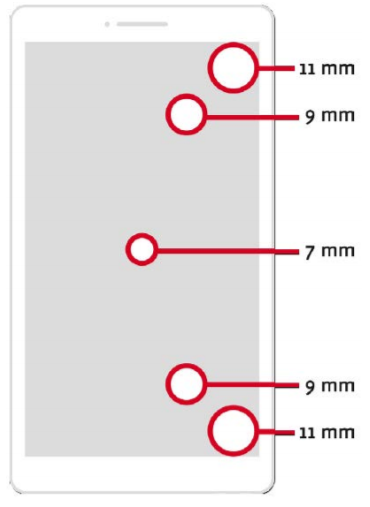
\includegraphics[width=0.3\textwidth]{img/dimvspos}
		\caption{Dimensione vs. posizione dei bottoni}
		\label{fig:dimvspos}
	\end{figure}
	
	\subsection{Menu}
	
	\begin{figure}[H] 
		\centering
		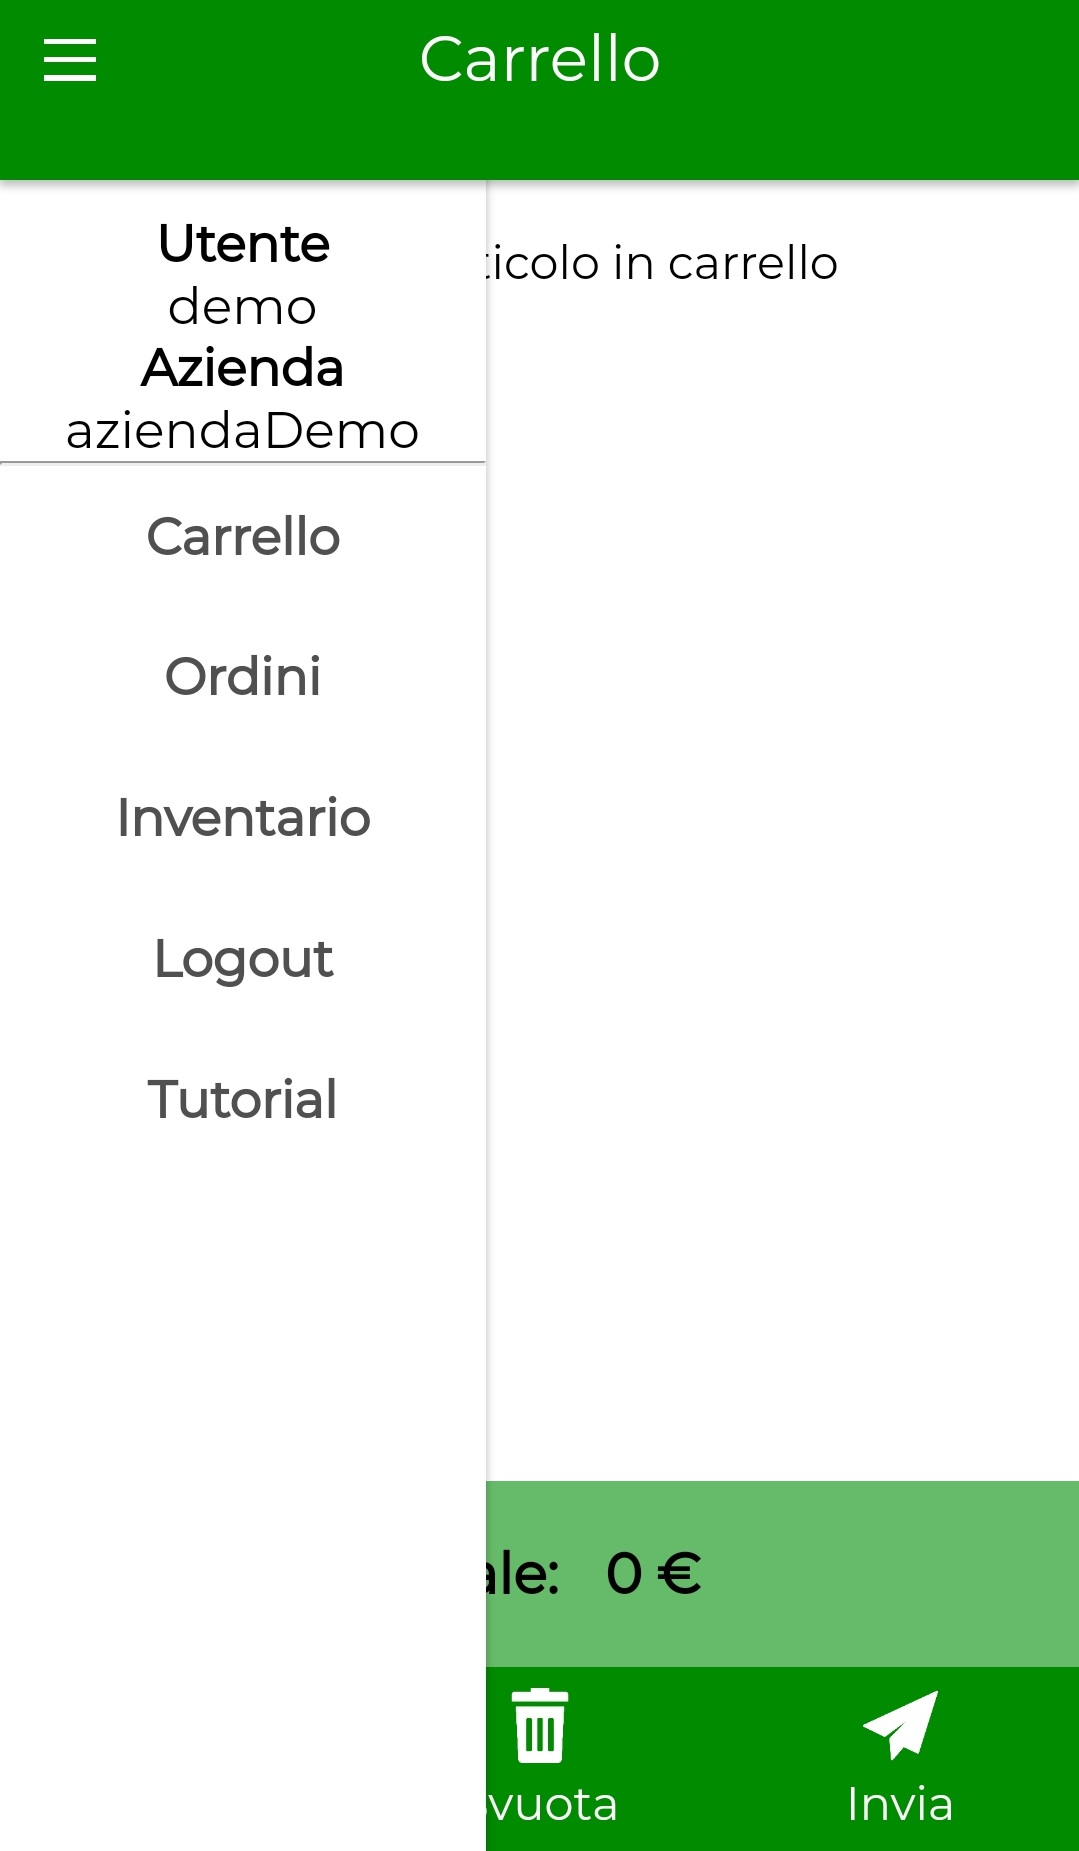
\includegraphics[width=0.3\textwidth]{img/menu}
		\caption{Menu dell'applicazione}
		\label{fig:menu}
	\end{figure}
	Il menu dell'applicazione è rappresentato in Figura \ref{fig:menu}. Per accederci è presente il classico bottone "hamburger" in alto a sinistra di ogni pagina. Il menu è suddiviso in due parti: 
	\begin{itemize}
		\item informazioni relative all'utente che ha effettuato il login nell'applicazione. In particolare vengono visualizzati il nome dell'utente e il codice azienda del fornitore dello stesso. Queste informazioni non sono modificabili e pertanto sono state disposte nella parte alta del menu;
		\item insieme di link che permettono di navigare tra le pagine dell'applicazione. In particolare sono disponibili i link al carrello, alla lista degli ordini e all'inventario. Inoltre è possibile effettuare il logout dall'applicazione o visionare nuovamente il tutorial. Questi bottoni sono stati posizionati nella parte centrale del menu (comfort zone), in modo da essere facilmente accessibili quando il menu risulta aperto.
	\end{itemize}

	\subsection{Progressive disclosure}
	
	In generale, è una buona prassi non affollare le interfacce. Al fine di perseguire questo obiettivo si è utilizzato il principio della progressive disclosure:
	\begin{itemize}
		\item nella pagina \textit{Ordini} è possibile visualizzare le informazioni essenziali per poter identificare un ordine. Per accedere ai dettagli risulta necessario un ulteriore tap;
		\item nella pagina \textit{Inventario} è possbile visualizzare le informazioni essenziali per poter identificare un articolo. Per accedere ai dettagli dello stesso, o per aggiungerlo al carrello, risulta necessario un ulteriore tap.
	\end{itemize}
	
	\subsection{Uso della tastiera}
	
	L'utilizzo della tastiera è necessario è stato limitato a tre casi:
	\begin{itemize}
		\item inseriremento delle credenziali in fase di login;
		\item ricerca di un articolo;
		\item inserimento o modifica della quantità nelle pagine \textit{Aggiungi} e \textit{Modifica}, rispettivamente. In questo caso la tastiera permette un veloce inserimento di grandi quantità.
	\end{itemize}
	Per l'inserimento della quantità è stata predisposta una seconda modalità. Sono stati messi a disposizione due pulsanti (+/-), i quali permettono di aumentare o diminuire la quantità, rispettivamente. Tramite questa modalità è possibile inserire velocemente piccole quantità.
	
	\subsection{Aiuti per l'utente}
	
	Al primo accesso di un utente all'applicazione, viene visualizzato il tutorial della stessa. Esso fornisce istruzioni rilevanti per l'utilizzo dell'applicazione e risulta breve, in quanto l'applicazione è stata progettata per essere massimamente intuitiva. Alla fine del tutorial è presente un bottone che permette di iniziare ad utilizzare l'applicazione. Il tutorial sarà comunque disponibile dal menu, nel caso in cui l'utente non ricordasse come utilizzare l'app.
	
	\subsection{Elementi nativi}
	
	Gli elementi nativi dell'applicazione sono la fotocamera, per la scansione del codice a barre, e i dialog, per la visualizzazione di messaggi informativi o di conferma. Per rendere questi elementi nativi si sono utilizzati i seguenti plugin di PhoneGap:
	\begin{itemize}
		\item dialogs: fornisce un'interfaccia per convertire gli alert e i confirm delle pagine web in dialog box nativi. In questo modo è stato possibile customizzare i titoli e le etichette dei pulsanti nei dialog;
		\item barcodescanner: fornisce un'interfaccia per accedere nativamente alla fotocamera del dispositivo ed effettuare la scansione di un codice a barre.
	\end{itemize}

	\subsection{Considerazioni sulla versione iOS}
	
	Nella versione iOS dell'applicazione è stato effettuato un solo cambiamento. Siccome sugli iPhone non esiste un tasto fisico o vistuale che permette di tornare indietro, si è dovuto aggiungere il classico pulsante indietro accanto al menu hamburger. È stata presa ispirazione per questa soluzione dall'applicazione di Amazon per iOS. Nel seguente screenshot è possibile vedere com'è stata implementata la soluzione.
	
	\subsection{Considerazioni finali}
	Si ritiene che l'applicazione soddisfi i primi tre livelli della piramide di Maslow rimappata sui bisogni degli utenti, ovvero che sia funzionale, affidabile e usabile.
	
	\section{Backend}
	Per l'implementazione del backend si è deciso di appoggiarsi ad Amazon AWS, in quanto tramite l'account universitario è possibile usufruire dei servizi offerti gratuitamente.
	\subsection{Architettura}
	Il backend della piattaforma presenta la seguente architettura:
	\begin{itemize}
		\item un server cloud Amazon AWS EC2 con installato Windows Server 2017;
		\item un'instanza Amazon AWS RDS contenente un database Microsoft SQL Server.
	\end{itemize}

	All'interno dell'istanza AWS EC2 sono stati installati:
	\begin{itemize}
		\item un server web Apache Tomcat: esso permette di eseguire un web service scritto in linguaggio Java, il quale si occupa di captare le richieste HTTP che provengono dall'applicazione, di elaborarle e di inviare delle risposte costruite sulla base di query effettuate su un database;
		\item il linguaggio Java: necessario per il funzionamento di Apache Tomcat e per l'esecuzione del web service.
	\end{itemize}

	\subsection{Web service}
	
	Per lo sviluppo del web service si sono utilizzati gli oggetti servlet Java. Essi permettono di captare richieste HTTP e di rispondere ad esse tramite stringhe in formato JSON. Il servizio web è costituito dai seguenti package:
	\begin{itemize}
		\item dbConnection: package contenente una classe utilizzabile per connettersi ed interagire con un database SQL Server;
		\item servlet: package contenente le classi servlet del servizio web;
		\item utility: package contenente le classi utilità del servizio web
	\end{itemize}

	\subsubsection{Servlet}
	
	In questa sezione vengono descritte le classi servlet e per ognuna di esse vengono indicate le seguenti caratteristiche:
	\begin{itemize}
		\item \textbf{End-point}: end-point che identifica il servlet. L'end-point è utilizzabile per comunicare con lo specifico servlet all'interno del web service;
		\item \textbf{Parametri}: lista dei parametri che devono essere inseriti nella richiesta HTTP per comunicare correttamente con il servlet;
		\item \textbf{Funzionalità}: una breve descrizione delle operazioni eseguite dal servlet e della tipologia di risposta che restituisce.
	\end{itemize}

	\begin{enumerate}
		\item \textbf{AggiuntaModificaArticolo.java}
		\begin{itemize}
			\item \textbf{End-point}: \textit{/AggiuntaModificaArticolo}
			\item \textbf{Parametri}:
			\begin{itemize}
				\item codice azienda: è il codice che identifica univocamente il database del fornitore corrispondente all'utente loggato;
				\item query: è la query di inserimento o modifica di un articolo nel carrello dell'utente loggato.
			\end{itemize}
			\item \textbf{Funzionalità}: il servlet si connette al database identificato dal codice azienda fornito ed effettua la query fornita su di esso. Se la query va a buon fine restituisce una stringa JSON contenente un messaggio positivo, altrimenti un messaggio negativo.
		\end{itemize}
	
		\item \textbf{Autenticazione.java}
		\begin{itemize}
			\item \textbf{End-point}: \textit{/Autenticazione}
			\item \textbf{Parametri}:
			\begin{itemize}
				\item username: è la username che l'utente ha inserito in fase di login;
				\item password: è la password che l'utente ha inserito in fase di login.
			\end{itemize}
			\item \textbf{Funzionalità}: il servlet si connette al database ideato per la gestione dell'autenticazione e cerca all'interno di esso le credenziali fornite. Se le credenziali vengono identificate viene resituita una stringa JSON contenente codice 0, altrimenti ci possono essere le seguenti possibilità:
			\begin{itemize}
				\item codice 1: la password inserita dall'utente non è quella corretta;
				\item codice 2: la username inserita dall'utente è inesistente.
			\end{itemize}
		\end{itemize}
	
		\item \textbf{EliminazioneArticoli.java}
		\begin{itemize}
			\item \textbf{End-point}: \textit{/EliminazioneArticoli}
			\item \textbf{Parametri}:
			\begin{itemize}
				\item username: è la username dell'utente loggato;
				\item codice azienda: è il codice che identifica univocamente il database del fornitore corrispondente all'utente loggato;
				\item lista codici: è la lista dei codici a barre dei prodotti che devono essere rimossi dal carrello dell'utente loggato.
			\end{itemize}
			\item \textbf{Funzionalità}: il servlet si connette al database identificato dal codice azienda fornito ed elimina dalla tabella \textit{contenutoCarrelli} gli articoli corrispondenti ai codici e alla username forniti. Infine restituisce una stringa JSON contenente codice 1 se l'eliminazione è andata a buon fine, altrimenti codice 0.
		\end{itemize}
	
		\item \textbf{InvioOrdine.java}
		\begin{itemize}
			\item \textbf{End-point}: \textit{/InvioOrdine}
			\item \textbf{Parametri}:
			\begin{itemize}
				\item username: è la username dell'utente loggato;
				\item codice azienda: è il codice che identifica univocamente il database del fornitore corrispondente all'utente loggato;
				\item totale: è il totale dell'ordine che l'utente ha deciso di inviare.
			\end{itemize}
			\item \textbf{Funzionalità}: il servlet si connette al database identificato dal codice azienda fornito e crea in database un nuovo ordine contenente gli articoli presenti nel carrello dell'utente identificato dalla username fornita. Infine invia una mail di notifica dell'ordine sia all'utente identificato dalla username fornito che all'azienda identificata dal codice azienda fornito.
		\end{itemize}
	
		\item \textbf{PrelevaArticoliAzienda.java}
		\begin{itemize}
			\item \textbf{End-point}: \textit{/PrelevaArticoliAzienda}
			\item \textbf{Parametri}:
			\begin{itemize}
				\item codice azienda: è il codice che identifica univocamente il database del fornitore corrispondente all'utente loggato;
			\end{itemize}
			\item \textbf{Funzionalità}: il servlet si connette al database identificato dal codice azienda fornito e restituisce una stringa JSON contenente le informazioni sugli articoli venduti dall'azienda.
		\end{itemize}
	
		\item \textbf{PrelevaDatiOrdine.java}
		\begin{itemize}
			\item \textbf{End-point}: \textit{/PrelevaDatiOrdine}
			\item \textbf{Parametri}:
			\begin{itemize}
				\item codice azienda: è il codice che identifica univocamente il database del fornitore corrispondente all'utente loggato;
				\item codice ordine: è il codice dell'ordine di cui si vogliono conoscere i dettagli.
			\end{itemize}
			\item \textbf{Funzionalità}: il servlet si connette al database identificato dal codice azienda fornito e restituisce una stringa JSON contenente le informazioni relative all'ordine corrispondente al codice ordine fornito.
		\end{itemize}
	
		\item \textbf{PrelevaOrdini.java}
		\begin{itemize}
			\item \textbf{End-point}: \textit{/PrelevaOrdini}
			\item \textbf{Parametri}:
			\begin{itemize}
				\item username: è la username dell'utente loggato;
				\item codice azienda: è il codice che identifica univocamente il database del fornitore corrispondente all'utente loggato;
			\end{itemize}
			\item \textbf{Funzionalità}: il servlet si connette al database identificato dal codice azienda fornito e restituisce una stringa JSON contenente le informazioni relative agli ordini effettuati dall'utente corrispondente alla username fornita.
		\end{itemize}
	
		\item \textbf{PrelievoInfoArticoli.java}
		\begin{itemize}
			\item \textbf{End-point}: \textit{/PrelievoInfoArticoli}
			\item \textbf{Parametri}:
			\begin{itemize}
				\item username: è la username dell'utente loggato;
				\item codice azienda: è il codice che identifica univocamente il database del fornitore corrispondente all'utente loggato;
			\end{itemize}
			\item \textbf{Funzionalità}: il servlet si connette al database identificato dal codice azienda fornito e restituisce una stringa JSON contenente le informazioni relative agli articoli nel carrello dell'utente identificato dalla username fornita.
		\end{itemize}
	
		\item \textbf{PrelievoInfoArticolo.java}
		\begin{itemize}
			\item \textbf{End-point}: \textit{/PrelievoInfoArticolo}
			\item \textbf{Parametri}:
			\begin{itemize}
				\item codice articolo: è il codice dell'articolo di cui si vogliono conoscere i dettagli;
				\item codice azienda: è il codice che identifica univocamente il database del fornitore corrispondente all'utente loggato;
			\end{itemize}
			\item \textbf{Funzionalità}: il servlet si connette al database identificato dal codice azienda fornito e restituisce una stringa JSON contenente le informazioni relative all'articolo corrispondente al codice articolo fornito.
		\end{itemize}
	\end{enumerate}
	
	\subsubsection{Utility}
	Il package \textit{utility} contiene le seguenti classi utilità:
	\begin{itemize}
		\item \textbf{GetDb}: classe contenente un metodo statico che restituisce la stringa di connessione dal database di autenticazione;
		\item \textbf{SendMail}: classe che fornisce un'interfaccia per l'invio di e-mail tramite un server SMTP Amazon AWS.
	\end{itemize}
	
	\subsection{Database}
	Per la gestione degli ordini, degli utenti e degli articoli venduti dai vari fornitori sono stati utilizzati dei database Microsoft SQL Server. In questa sezione vengono descritti i seguenti database:
	\begin{itemize}
		\item database di autenticazione;
		\item database aziendale.
	\end{itemize}
	
	\subsubsection{Database per l'autenticazione}
	Il database per l'autenticazione contiene le credenziali e le anagrafiche degli utenti registrati e le informazioni dei fornitori registrati all'applicazione. Questo database contiene le seguenti tabelle:
	\begin{itemize}
		\item aziende: contiene le informazioni delle aziende registrate a SmartOrder. La tabella contiene i seguenti attributi:
		\begin{itemize}
			\item codAzienda (chiave primaria): è un codice che identifica univocamente l'azienda. Esso viene fornito all'azienda in fase di registrazione all'applicazione;
			\item nome: è il nome dell'azienda;
			\item via: è la via dove è situata la sede principale dell'azienda;
			\item civico: è il civivo dove è situtata la sede principale dell'azienda;
			\item comune: è il comune dove è situata la sede principale dell'azienda;
			\item provincia: è la provincia dove è situata la sede principale dell'azienda;
			\item CAP: è il codice postale dove è situata la sede principale dell'azienda;
			\item mail: è la mail che l'azienda ha fornito in fase di registrazione;
			\item telefono: è il numero di telefono che l'azienda ha fornito in fase di registrazione.
		\end{itemize}
		\item users: contiene le informazioni relative agli utenti registrati a SmartOrder. La tabella contiene i seguenti attributi:
		\begin{itemize}
			\item username (chiave primaria): è il nome utente che è stato fornito all'utente in fase di registrazione;
			\item password: è la password che è stata fornita all'utente in fase di registrazione;
			\item mail: è la mail che l'utente ha fornito in fase di registrazione;
			\item codAzienda: è il codice dell'azienda presso cui l'utente è cliente;
			\item cellulare: è il numero di cellulare che l'utente ha fornito in fase di registrazione;
			\item nome: è il nome dell'utente;
			\item cognome: è il cognome dell'utente;
			\item via: è la via di residenza dell'utente;
			\item civico: è il civico di residenza dell'utente;
			\item comune: è il comune di residenza dell'utente;
			\item provincia: è la provincia di residenza dell'utente;
			\item CAP: è il codice postale di residenza dell'utente.
		\end{itemize}
	\end{itemize}
	
	\subsubsection{Database aziendale}
	Il database aziendale contiene le informazioni relative agli articoli venduti e agli ordini effettuati presso uno specifico fornitore. Per cui nel server è presente un database di questa tipologia per ogni fornitore registrato all'applicazione. Questo database contiene le seguenti tabelle:
	\begin{itemize}
		\item articoli: contiene le informazioni relative agli articoli venduti dall'azienda. La tabella contiene i seguenti attributi:
		\begin{itemize}
			\item nome: è il nome dell'articolo;
			\item barCode (chiave primaria): è il codice a barre dell'articolo;
			\item prezzo: è il prezzo dell'articolo;
			\item descrizione: è la descrizione dell'articolo.
		\end{itemize}
		\item contenutoCarrelli: contiene le informazioni relative al contenuto dei carrelli degli utenti dell'azienda. La tabella contiene i seguenti attributi:
		\begin{itemize}
			\item idRiga (chiave primaria): è un identifico autoincrementante che funge unicamente da chiave primaria;
			\item barCode: è il codice a barre dell'articolo in carrello;
			\item quantità: è la quantità scelta dall'utente per l'articolo in carrello;
			\item username: è lo username dell'utente che ha inserito in carrello l'articolo.
		\end{itemize}
		\item contenutoOrdini: contiene le informazioni relative al contenuto degli ordini effettuati presso l'azienda. La tabella contiene i seguenti campi:
		\begin{itemize}
			\item idRiga (chiave primaria): è un identifico autoincrementante che funge unicamente da chiave primaria;
			\item codiceOrdine: è il codice dell'ordine in cui é presente l'articolo;
			\item barCode: è il codice a barre dell'articolo all'interno dell'ordine;
			\item quantità: è la quantità ordinata per l'articolo.
		\end{itemize}
		\item ordini: contiene le informazioni relative agli ordini effettuati presso l'azienda. La tabella contiene i seguenti campi:
		\begin{itemize}
			\item codiceOrdine (chiave primaria): è il codice che identifica univocamente l'ordine presso l'azienda;
			\item data: è la data in cui l'ordine è stato effettuato;
			\item username: è la username dell'utente che ha effettuato l'ordine;
			\item totale: è il totale in euro dell'ordine.
		\end{itemize}
	\end{itemize}
	
	\section{Conclusioni}
	Vi è la consapevolezza che l'interfaccia grafica poteva essere resa più accattivante per lo scopo dell'applicazione. L'implementazione della stessa poteva risultare più semplice tramite l'utilizzo di un altro framework, come ad esempio React Native. 
	Il framework scelto ha comunque permesso di realizzare una buona interfaccia grafica in tempi ristretti. Vi è la consapevolezza che un framework ibrido non dovrebbe essere la prima scelta nel caso si utilizzino i sensori del dispositivo (fotocamera in questo caso). Per giustificare la scelta di PhoneGap si ritiene che il tempo necessario per l'apprendimento delle tecnologie richieste dagli altri framework sia di gran lunga superiore e non avrebbe permesso al gruppo di consegnare il progetto alla consegna pianificata. Infatti erano stati presi in considerazione i framework \textit{Xamarin} e \textit{React Native}, i quali richiedevono l'apprendimento di \textit{C#} e \textit{React}, rispettivamente, linguaggi totalmente sconosciuti dai membri del gruppo. Nonostante questo problema il gruppo ritiene di aver realizzato una buona applicazione, che potrebbe risultare utile ad aziende ed utenti nel contesto per cui è stata progettata e implementata.
\end{document}